\cleartooddpage[\thispagestyle{empty}]
\chapter{Analysis}\label{chapter:analysis}

\section{Veritas Data}\label{veritasdata}
  The analysis in this thesis relies on three sets of VERITAS data.
  One set observes the Crab Nebula, another observed the Galactic Center, and a third set observes a dark region \SI{5}{\degree} NW of the Galactic Center.
  This dark region is referred to as  Sgr A* Off, and is located at (l,b)=(\SI{357.3396}{\degree}, \SI{3.9984}{\degree}), shown in Figure \ref{fig:gcfieldsofview}.

  \begin{figure}[ht]
    \centering
    \includegraphics[width=0.95\textwidth]{images/skypointings/plot.eps}
    \caption[VERITAS Galactic Center Pointings]{
      Fields of view for Galactic Center observations.
      Each circle marks the detection area of one observation.
      Green circles are data observations, while blue circles are dark observations used to construct the camera-background templates.
      To quantify the detector efficiency, observations are taken at \SI{0.5}{\degree} or \SI{0.7}{\degree} offsets from each observing target, in four different directions (wobbles) along Right Ascension/Declination axes.
    }
    \label{fig:gcfieldsofview}
  \end{figure}

  %2 offsets $\times$ 4 wobble directions = 8 observing regions (circles).

  All three sets of data include observations from both the V5 epoch (after moving T4 but before the camera upgrade), and the V6 epoch (after the camera upgrade).
  All used data was taken from April 2010 to June 2016.

  %
  % times calculated with $VERIPY/thesis/plots/obs_times.py
  %
  \begin{table}[]
    \centering
    \caption{Hours of observations taken at each source/epoch combination.}
    \label{tab:observation_times}
    \begin{tabular}{|l|l|l|l|}
      \hline
      \textbf{Epoch} & \textbf{Crab} & \textbf{Sgr A*} & \textbf{Sgr A* Off} \\ \hline
      V5             & 3.3           & 46.3            & 13.0                \\ \hline
      V6             & 5.5           & 62.7            & 4.7                 \\ \hline
    \end{tabular}
  \end{table}


  \begin{figure}[ht]
    \centering
    \includegraphics[width=0.95\textwidth]{data_elevation_plots/plot.eps}
    \caption[VERITAS Data Elevation Exposure]{
      Camera center elevation for the three sets of data.
      The three peaks in the Sgr A* data are from the 4 wobble positions being at different elevations.
      The North wobble observations peak at elevation \nicetilde29.75\degree, East and West wobbles observations at \nicetilde29.25\degree, and South wobble observations at \nicetilde28.75\degree.
    }
    \label{fig:datapointingelevations}
  \end{figure}

  There are comparativly fewer Sgr A* Off observations, as there are no gamma-ray emitters at or near that position, and telescope time is valuable.
  There is also even fewer Crab observations, as the majority of its observations are done at higher elevations, where the telescope is more sensitive to lower energies.
  
  For all of these observations, quality checks were applied.
  This includes monitoring the telescope hardware and weather by a team of VERITAS collaboration members who take the observations.
  After the data is taken, a separate collaboration member will go through each observation to check it again, and mark any bad observations or apply time cuts, which are then removed.

  As multiple studies in the past have shown that the different VERITAS epochs perform differently, each epoch has their own separate set of effective areas, point spread functions, energy migration matricies, and camera background models.
  In addition, specific IRFs were calculated for additional data dimensions, including the frequency of night sky background photons in the camera, the telescope elevation, the event energy, and each event's distance from the camera center.

\section{Likelihood Ratio Test}
  The likelihood ratio test is a method of comparing whether a function is a statistically preferable fit to some data, compared to another function.
  This ratio test performed by calculating the test statistic (TS) for a set of data and two functions of that data ($M_{\text{null}}$ and $M_{\text{alt}}$), shown in Equation \ref{eqn:test_statistic}.
  
  % from https://arxiv.org/pdf/1606.00393.pdf, equation 50
  \begin{equation}\label{eqn:test_statistic}
    \text{TS} = 2 \, \text{ln} \, L \left(M_{\text{alt}} \right ) - 2 \, \text{ln} \, L \left( M_{\text{null}} \right )
  \end{equation}
  
  The function $L$ is the likelihood of each model, calculated via summing the likelhiood of individual observations $L_i$ in Equation \ref{eqn:sum_likelihood}.
  
  % from https://arxiv.org/pdf/1606.00393.pdf, equation 6
  \begin{equation}\label{eqn:sum_likelihood}
    - \text{ln} \, L \left(M \right ) = - \sum_i \text{ln} \, L_i \left(M \right )
  \end{equation}
  
  The two functions $M_{\text{null}}$ and $M_{alt}$ are sometimes referred to as hypotheses.
  For the unbinned statistical comparison used in this analysis, the likelihood $L$ of each function $M$ is computed via Equation \ref{eqn:unbinned_likelihood}.
  
  % from https://arxiv.org/pdf/1606.00393.pdf, equation 1
  \begin{equation}\label{eqn:unbinned_likelihood}
    - \text{ln} \, L_i \left ( M \right ) = e_i \left ( M \right ) - \sum_k \text{ln} \, P_i \left ( \boldsymbol{p}'_k, E'_k, t'_k \, | \, M \right )
  \end{equation}
  
  Where $i$ is the $i^{\text{th}}$ observation, also referred to as a chunk in Section \ref{fitsconversion}.
  $k$ is the $k^{\text{th}}$ event in the observation, $\boldsymbol{p}'_k$ is the reconstructed event point-of-origin, $E'_k$ is the reconstructed event energy, and $t'_k$ is the event arrival time.
  The primed $\boldsymbol{p}'$, $E'$, and $t'$ denote the reconstructed (detector) quantities, which are separate from the true (sky) $\boldsymbol{p}$, $E$, and $t$ quantities.
  The function $P$ is the poissonian probability of getting an event with properties $\boldsymbol{p}'$, $E'$, and $t'$, given the hypothesis $M$, shown in Equation \ref{eqn:probability_summation}.
  
  % from https://arxiv.org/pdf/1606.00393.pdf, equation 7
  \begin{equation}\label{eqn:probability_summation}
  P_i \left ( \boldsymbol{p}', E', t' | M \right ) = \sum_j P_i \left ( \boldsymbol{p}', E', t' | M_j \right )
  \end{equation}

  Where $M_j$ is the $j^{\text{th}}$ model within hypothesis $M$.
  Each hypothesis contains one camera background model (Section \ref{background_production}) per chunk (Section \ref{fitsconversion}), plus any astrophysical models.
  $P_i \left( \boldsymbol{p}', E', t' | M_j \right )$ is the probability of getting an event from a single astrophysical model $M_j$, depicted in Equation \ref{eqn:single_probability}.
  
  % from https://arxiv.org/pdf/1606.00393.pdf, equation 8
  \begin{equation}\label{eqn:single_probability}
    P_i \left ( \boldsymbol{p}', E', t' | M \right ) = \int_{ \boldsymbol{p},E,t} R_i \left( \boldsymbol{p}',E',t'| \boldsymbol{p},E,t \right ) \times M_j^S \left( \boldsymbol{p}, E, t \right ) d\boldsymbol{p} \, dE \, dt
  \end{equation}
  
  While for a detector model (like the background models), $P_i$ is calculated via:
  
  % from https://arxiv.org/pdf/1606.00393.pdf, equation 9
  \begin{equation}
    P_i \left ( \boldsymbol{p}', E', t' | M_j \right ) = M^D_{j,i} \left ( \boldsymbol{p}', E', t' \right )
  \end{equation}
  
  Where:

  % from https://arxiv.org/pdf/1606.00393.pdf, equation 10
  \begin{equation}
    M^S \left ( \boldsymbol{p}, E, t \right ) = M_S \left ( \boldsymbol{p}|E,t \right ) \times M_E \left ( E | t \right ) \times M_T \left ( t \right )
  \end{equation}
  
  {\color{red} Explain better what these three equations are??  what is $R_i$??}
  
  Equation \ref{eqn:single_probability} is formed by convolving the predicted number of counts from the model with the detector dispersion function $R$.
  
  In Equation \ref{eqn:unbinned_likelihood}, $e_i \left ( M \right )$ is the predicted number of events from hypothesis $M$, detailed in Equation \ref{eqn:model_integration}.

  % from https://arxiv.org/pdf/1606.00393.pdf, equation 2
  \begin{equation}\label{eqn:model_integration}
    e_i \left(M \right ) = \int_{GTI} \int_{Ebounds} \int_{ROI} P_i \, \left( \boldsymbol{p}', E', t' \, | \, M \right ) d\boldsymbol{p}' \, dE' \, dt'
  \end{equation}
  
  This is calculated via integrating over each observation's live time window (the Good Time Interval or $GTI$), the reconstructed energy range ($Ebounds$), and the spatial Region Of Interest ($ROI$).
  
  
  The likelihood ratio test useful for comparing two hypotheses.
  They are referred to as the null and alternative hypotheses.
  Each hypothesis consists of a collection of models, where each model predicts the number of events at each point in the energy/space/time parameter space.
  Once each hypothesis is constructed, the likelihood for each can be computed.
  
  {\color{red}likelihood equation??}
  
  
  The ratio of the two likelihoods then follows a gaussian (with certain assumptions), meaning the sigificance of the alternative hypothesis over the null can be calculated.
  As part of this likelihood ratio test, the signal and background models must be constructed.
  Background models can be camera background models (discussed in section \ref{sec:bkgmodels}), or astrophysical models of background gamma-ray emitters.

  {\color{red}test statistic equation??}

\section{Background Models}\label{sec:bkgmodels}
  The background models predict the amount of background counts produced by a gamma-ray-empty sky.
  This is used to model the effect of the background (primarily proton) events, which are several orders of magnitude more populous than the gamma rays.
  Producing the backgrounds is performed by binning observation sources with weak or no gamma-ray emission.
  For this low-elevation analysis, special observation runs were taken several degrees away from the galactic center (see Figure \ref{fig:gcfieldsofview}).

  These background runs were then assembled into background models via the procedure in subsection \ref{background_production}.
  To account for the difference between the V5 and V6 observatory configurations, the background observations are divided up based on their epoch, producing unqiue backgrounds for each epoch.
  These background templates vary with respect to the radial distance from the camera center, and the event energy.

  To confirm that these background models fit properly, a simple likelihood analysis was performed with the Off observations and their backgrounds.
  If the background models were assembled astutely, after the liklelihood normalization, the number of events observed and predicted by the models is shown in {\color{red}figure ??}.

  {\color{red}(using just the background observations, show profile plots in galactic-b and energy??)}

\section{Test Point Sources}
  To verify that the CTOOLs likelihood analysis is working properly, two point sources were analyzed first, before any dark matter analysis was performed.
  The first was on the well-studied Crab nebula, and the second was on the source at the center of our galaxy.
  To also uncover any low-elevation effects, the Crab observations were limited to ones with elevations < \SI{32.5}{\degree} (see Figure \ref{fig:datapointingelevations}).

  {\color{red}(plot of Crab, Sgr A*, Sgr A* Off sources elevations??)}

  \subsection{Test Crab Analysis}\label{subsec:crab_analysis}

    In order to test that the converted data, irfs, and ctools likelihood engine all work properly, a test analysis on the Crab nebula was performed.
    As the Crab nebula is the brightest gamma ray emitter in the sky, it has been observed extensively by VERITAS and other gamma ray telescopes.
    Since the Galactic Center only rises to around \SI{30}{\degree} elevation, elevation effects would also need to be searched for.
    After searching for low-elevation Crab observations, a total of 17.1 hours of livetime were found.
    These consist of 7.3 {\color{red}(doesn't match with plot??)} hours of V5 epoch data, and 9.8 {\color{red}(doesn't match with plot??)} hours of V6 epoch data.
    
    \begin{figure}[h]
      \centering
      \includegraphics[width=0.95\textwidth]{images/test_crab_analysis/plot_elev27_5_32_5deg_4_70TeV_wobbleall_Epochall_skymap.eps}
      \caption[Crab Counts Skymap]
      {
        Skymap of event positions.
        No corrections are made for observing time or effective area.
      }
      \label{fig:crab_skymap}
    \end{figure}
    
    The Crab was modeled by a single point source with a simple power law spectrum:

    \begin{equation} \label{eqn:powerlaw}
    F\left( E \right) = I_{0} \left( \frac{E}{E_{0}} \right)^{-\gamma}
    \end{equation}

    Only events between 4 and 70 TeV are used in this test analysis.
    At an elevation of 25\degree, the reconstruction software is able to reconstruct events as low as 1.5 TeV.
    But, in this 'threshold' energy region, the camera sensitivity starts to decrease in a poorly understood way, and IRFs in this region are not accurate.
    Part of this decrease is explored in section (see figures \ref{fig:bkgvsel_crab} and \ref{fig:bkgvsel_sgra}), but implementing corrections requires large changes to existing code, along with a larger set of simulations, neither of which were feasible during this work.
    Above 70 TeV, simulations become too computationally expensive to create when attempting to calculate IRFs.
    
    After fitting all events from \SI{4}{TeV} to \SI{70}{TeV}, with a pivot energy $ E_{0}= \SI{10}{TeV} $, the $ I_{0} = \left(1.472\pm0.09\right)*10^{-19} \frac{ph}{cm^{2} s MeV} $, $ \gamma = 2.382 \pm 0.076 $, with a Test Statistic of 1929.01. {\color{red}(?? update values!)}.
    As the crab (alternative) hypothesis has 110 free parameters, and the no-crab (null) hypothesis has 108 free parameters, the Test Statistic has $ 110 - 108 = 2 $ degrees of freedom.
    This is roughly equivalent to a {\color{red}significance of ??}.
    
    In the standard VERITAS Eventdisplay analysis, the crab is found to have a point source significance of \SI{21.3}{$\sigma$}.
    
    
    \begin{figure}[h]
      \centering
      \includegraphics[width=0.95\textwidth]{images/test_crab_analysis/plot_elev27_5_32_5deg_4_70TeV_wobbleall_Epochall.eps}
      \caption[Crab Test Spectrum]
      {
        Crab spectra from various analyses and observatories.
        Red is the spectra from the CTOOLS analysis described in this chapter.
        Blue is the standard VERITAS Eventdisplay spectrum using the same set of observations.
        {\color{red}(Update hess/magic lines to have higher maximum energy points??)}
      }
      \label{fig:crab_test_spectra}
    \end{figure}
    
    In figure \ref{fig:crab_test_spectra}, the fitted crab spectra is shown, along with literature results from earlier VERITAS, HESS, and MAGIC observations of the Crab.
    
    \begin{figure}[h]
      \centering
      \includegraphics[width=0.95\textwidth]{images/test_crab_analysis/plot_elev27_5_32_5deg_4_70TeV_wobbleall_Epochall_spl.eps}
      \caption[Crab Profile along Galactic L]
      {
        The number of counts along a \SI{0.16}{\degree}-wide-slice through the Crab along the Galactic L axis.
        Blue points are the number of observed counts, with poissonian error bars.
        The green histogram bars are the number of counts predicted by all models.
        Purple histogram bars are the number of counts predicted by only the camera-background models.
        The dark green line is a high-resolution version of the green histogram.
      }
      \label{fig:crab_profile_l}
    \end{figure}

    \begin{figure}[h]
      \centering
      \includegraphics[width=0.95\textwidth]{images/test_crab_analysis/plot_elev27_5_32_5deg_4_70TeV_wobbleall_Epochall_spb.eps}
      \caption[Crab Profile along Galactic B]
      {
        The number of counts along a \SI{0.16}{\degree}-wide-slice through the Crab along the Galactic B axis.
        Blue points are the number of observed counts, with poissonian error bars.
        The green histogram bars are the number of counts predicted by all models.
        Purple histogram bars are the number of counts predicted by only the camera-background models.
        The dark green line is a high-resolution version of the green histogram.
      }
      \label{fig:crab_profile_b}
    \end{figure}
    
    \begin{figure}[h]
      \centering
      \includegraphics[width=0.95\textwidth]{images/test_crab_analysis/plot_elev27_5_32_5deg_4_70TeV_wobbleall_Epochall_splalt.eps}
      \caption[Crab Profile along Galactic L Off Source]
      {
        The number of counts along a \SI{0.16}{\degree}-wide-slice along the Galactic L axis.
        This slice doesn't go through the Crab, but instead \SI{1}{\degree} higher in Galactic B.
        As this doesn't include the Crab, this plot primarily demonstrates the camera background modelling.
        Blue points are the number of observed counts, with poissonian error bars.
        The green histogram bars are the number of counts predicted by all models (not visible as the astrophysical crab model doesn't contribute any amount of counts in this offset slice).
        Purple histogram bars are the number of counts predicted by only the camera-background models.
        The dark green line is a high-resolution version of the green histogram.
      }
      \label{fig:crab_profile_l_off}
    \end{figure}

    \begin{figure}[h]
      \centering
      \includegraphics[width=0.95\textwidth]{images/test_crab_analysis/plot_elev27_5_32_5deg_4_70TeV_wobbleall_Epochall_ep.eps}
      \caption[Crab Profile in Energy]
      {
        The number of counts in a \SI{0.6}{\degree} x \SI{0.6}{\degree} square centered on the Crab, vs energy.
        Blue points are the number of observed counts, with poissonian error bars.
        The green histogram bars are the number of counts predicted by all models.
        Purple histogram bars are the number of counts predicted by only the camera-background models.
      }
      \label{fig:crab_profile_energy}
    \end{figure}
    
    The fitted models can also be viewed, as a check that the likelihood engine is fitting the models to the data.
    In figure \ref{fig:crab_skymap}, the position of all counts is shown in galactic l and b.
    In figures \ref{fig:crab_profile_l} and \ref{fig:crab_profile_b}, the counts in the observations and models were integrated along a slice of galactic l and b.
    The counts from only the camera background models is shown, along with the counts from all camera backgrounds plus the point source.
    The difference between these two lines is then the counts from the Crab point source model.
    In figure \ref{fig:crab_profile_energy}, a similar plot is made, though integrated in a \SI{0.6}{\degree}x\SI{0.6}{\degree} square around the crab at different energies.

\section{Dark Matter Likelihood Analysis}
  \subsection{Non-Dark-Matter Models}
  For this analysis, a point source model was added at the position of Sgr A*.
  This is because other analyses (\cite{gc_pnt_is_not_dm1}, \cite{gc_pnt_is_not_dm2}, and \cite{gc_pnt_is_not_dm3} {\color{red}read these to double-check they lean away from a dm source??}) have indicated that the bright gamma-ray source at Sgr A* is not consistant with a dark matter halo.
  Instead, a point source with a broken power law spectrum (Equation \ref{eqn:brokenplaw}) is added to the list of models, with the magnitude of its flux left free by the likelihood engine.
  
  \begin{equation}\label{eqn:brokenplaw}
    \frac{dN}{dE} = N_{0} * { \left ( \frac{E}{E_{pivot}} \right ) }^{\alpha} {e}^{-\frac{E}{E_{cut}}}
  \end{equation}
  
  From \cite{VeritasGCRidge2015}, the specific values used in this point source were $E_{pivot}=\SI{1}{TeV}$, $E_{cut}=\SI{12.8}{TeV}$, and $\alpha=-2.1$.
  The normalization $N_{0}$ was initially set to $2.8*{10}^{-12}\,\text{cm}^{-2}\,\text{s}^{-1}\,\text{TeV}^{-1}$, but was left free in the likelihood optimization, while $E_{pivot}$, $E_{cut}$, and $\alpha$ were all fixed.
  The normalization was left free to allow for the potential of some mixing between the point source events and any dark matter halo events, i.e. a stronger dark matter halo gamma-ray flux would result in a weaker point source flux.
  
  Diffuse emission, eliminated due to complexity?

  \subsection{Dark Matter Models}
  Dark Matter halos are modeled by a spherically-symmetric mass-per-volume density profile.
  In this analysis, an Einasto density profile (discussed in section \ref{dm_spatial}) is used as the spatial component of the dark matter halo model.
  For the spectral component, each dark matter mass tested has its own spectrum produced with CLUMPY (see section \ref{dm_spectral}).

  \subsection{Likelihood Results}
  
  A histogram of all observed events is shown in figure \ref{fig:gc_counts_skymap}.
  
  \begin{figure}[ht]
    \centering
    \includegraphics[width=0.95\textwidth]{images/likelihood_analysis/counts_skymap.eps}
    \caption[Galactic Center Counts Skymap]{
      Skymap of all event positions used in this analysis.
      No adjustment for effective area, observation time, or background rate is done here.
      {\color{red}Veritas->VERITAS}
    }
    \label{fig:gc_counts_skymap}
  \end{figure}

  An energy histogram of all events from \SI{4}{TeV}-\SI{70}{TeV} is shown in figure \ref{fig:gc_counts_enhist}.
  
  \begin{figure}[ht]
    \centering
    \includegraphics[width=0.95\textwidth]{images/likelihood_analysis/counts_enhist.eps}
    \caption[Galactic Center Counts Energy Histogram]{
      Histogram of all event positions used in this analysis.
      No adjustment for effective area, observation time, or background rate is done here.
      {\color{red}(Fix x axis range and tick labels (rerun halo.py!) ??)}
    }
    \label{fig:gc_counts_enhist}
  \end{figure}

  The analysis uses the $b\bar{b}$ annihilation channel, and are shown for just at \SI{45}{TeV}.

  In figure \ref{fig:gc_profile_gal_l}, the observed counts are shown compared to the final, likelihood-optimized modelled counts.
  The histogram bins are along a 0.22\degree-wide slice along the galactic l axis, centered on Sgr A*'s galactic b coordinate.
  The purple histogram bins are the modelled counts from only the camera background models.
  The green histogram bins are the total modelled counts from the camera background models and the astrophysical models.
  The blue points with error bars are the observed counts in each bin, with poissonian errors.
  The lighter green line is a higher-resolution sampling of the total modelled counts.
  The feature where the observed counts are shifted to the left of the models is likely due to unaccounted-for elevation effects in the camera background models.
  
  \begin{figure}[h]
    \centering
    \includegraphics[width=0.95\textwidth]{images/likelihood_analysis/profile_gal_l.eps}
    \caption[Galactic Center Profile vs Galactic L]{
      Observed vs modeled counts in a slice of the sky parallel to the galactic L axis at $B=0$.
      Modeled counts from camera-background-models are shown in purple, total modeled counts are shown in green.
      The faint green line shows the total modelled counts at a higher spatial resolution, scaled to the histogram bins.
      Observed counts with poissonian errors are shown in blue.
    }
    \label{fig:gc_profile_gal_l}
  \end{figure}

  Figure \ref{fig:gc_profile_gal_b} is almost the same as figure \ref{fig:gc_profile_gal_l}, except it is a slice through Sgr A* along the galactic b axis,
  The feature where the observed counts are shifted to the left of the models is also visible here.

  \begin{figure}[h]
    \centering
    \includegraphics[width=0.95\textwidth]{images/likelihood_analysis/profile_gal_b.eps}
    \caption[Galactic Center Profile vs Galactic B]{
      Observed vs modeled counts in a slice of the sky parallel to the galactic B axis at $L=0$.
      Modeled counts from camera-background-models are shown in purple, total modeled counts are shown in green.
      Observed counts with poissonian errors are shown in blue.
    }
    \label{fig:gc_profile_gal_b}
  \end{figure}

  Figure \ref{fig:gc_profile_energy} shows the same profile, except instead integrated over a ${0.2}^{\circ}\times{0.2}^{\circ}$ galactic (l,b) square centered on Sgr A*.
  Again, purple is modelled camera-background counts, green is total modelled counts, and blue is observed counts.
  
  \begin{figure}[h]
    \centering
    \includegraphics[width=0.95\textwidth]{images/likelihood_analysis/profile_energy.eps}
    \caption[Galactic Center Profile vs Energy]{
      Observed vs modeled counts in a ${0.2}^{\circ}\times{0.2}^{\circ}$ square bin centered on Sgr A* at energies from \SI{4}{TeV} to \SI{70}{TeV}.
      Modeled counts from camera-background-models are shown in purple, total modeled counts are shown in green.
      Observed counts with poissonian errors are shown in blue.
    }
    \label{fig:gc_profile_energy}
  \end{figure}
  
  To check for any poorly modelled areas of the sky, a residual skymap is shown in figure \ref{fig:gc_resmap}.
  This calculates how significant the difference is between the observed and modelled number of counts.
  Each bin's significance is 
  
  % see http://cta.irap.omp.eu/ctools/users/reference_manual/csresmap.html
  \begin{equation}
    \label{eqn:resmap_signif}
    \text{Significance} = sign(D-M) \sqrt{ 2 \left ( D * ln \left ( \frac{D}{M} \right ) + M - D \right ) }
  \end{equation}
  
  where D is the number of observed counts, and M is the number of modelled counts.
  Equation \ref{eqn:resmap_signif} is derived from the Li and Ma {\color{red}equation ??}. 
  In this plot, the deficiency of the radially-symmetric camera background models is apparent.
  Lighter/darker areas indicate places where there were more/less observed counts than the models predicted.
  
  \begin{figure}[ht]
    \centering
    \includegraphics[width=0.95\textwidth]{images/likelihood_analysis/plot_resmap_algosignificance.eps}
    \caption[Galactic Center Residual Map]
    {
      Significance of each skymap bin's residual counts.
      See equation \ref{eqn:resmap_signif} for details.
      The dark upper-left and lighter lower-right areas are due to the the radiall-symmetric background, when a non-radially symmetric one would have been more ideal.
    }
    \label{fig:gc_resmap}
  \end{figure}

  Even if the source and background models were perfectly known, there would still be statistical fluctuations in the observed counts, and the residual significances would form a gaussian distribution, shown as the green line in figure \ref{fig:gc_resmap_sighist}.
  However, the distribution of the pixel significances from figure \ref{fig:gc_resmap} is shown in figure \ref{fig:gc_resmap_sighist}, and qualitativly not gaussian shaped {\color{red}(??)}.
  {\color{red}?? How well does it fit, and quantitativly how bad does it fit??}
  As a large number of bins are clustered around +2 and -2 signifiance, this hints that the residuals in figure \ref{fig:gc_resmap} are potentially not due solely from statistical noise, and that the background modelling could be improved.
  
  \begin{figure}[ht]
    \centering
    \includegraphics[width=0.95\textwidth]{images/likelihood_analysis/plot_resmap_phist_algosignificance.eps}
    \caption[Galactic Center Residual Histogram]
    {
      Histogram of the residual skymap bin significances from figure \ref{fig:gc_resmap}.
      See equation \ref{eqn:resmap_signif} for details.
      Only skymap bins within each observation's region of interest (the green circles in figure \ref{fig:gcfieldsofview}) are histogrammed.
    }
    \label{fig:gc_resmap_sighist}
  \end{figure}
  
\section{Upper Limit}
  An upper limit on the flux of a source can be calculated by scaling the flux of a model until the log-likelihood is at the 0.95 confidence level.
  This is done by using the ctulimit tool in ctools.
  
  Then from the dark matter flux {\color{red}equation ??}, an upper limit on the observed gamma-ray flux can be used to calculate an upper limit on the velocity-averaged crosssection.
  
  \begin{equation}\label{eqn:ulim}
    \frac{d\phi}{dE d\Omega} = \frac{ \left \langle \sigma v \right \rangle }{8\pi m_{\chi}^{2}} \frac{dN_{\gamma}}{dE} \int \rho^{2} dl
  \end{equation}
  
  Since, when all other variables are fixed, a larger gamma ray flux results from a larger velocity-averaged crosssection, they can both be replaced with their upper limits {\color{red}(??)}.

  \begin{figure}[ht]
    \centering
    \includegraphics[width=0.95\textwidth]{images/ulimit/final_upper_limit_plot.eps}
    \caption[Dark Matter Upper Limit Plot]{
      Dark Matter upper limits on velocity-averaged cross-sections.
      For reproduction, data values from this work {\color{red}are in table ??}.
    }
    \label{fig:ulim}
  \end{figure}
  
\section{Systematic Errors}  

Stuff?


